\documentclass[12pt]{beamer}
\usepackage{../latex-sty/mypres}
\usepackage[utf8]{inputenc}
\usepackage[T2A]{fontenc}
\usepackage[english]{babel}

\expandafter\def\expandafter\insertshorttitle\expandafter{%
  \insertshorttitle\hfill%
  \insertframenumber\,/\,\inserttotalframenumber}
\title[Seminar 9]{Optimization methods. \\
 Seminar 9. Conjugate functions}
\author{Alexandr Katrutsa}
\institute{Moscow Institute of Physics and Technology\\
Department of Control and Applied Mathematics} 
\date{\today}

\begin{document}
\begin{frame}
\maketitle
\end{frame}

\begin{frame}{Reminder}
\begin{itemize}
\item Feasible direction cone
\item Tangent cone
\item Sharp extremum 
\end{itemize}
\end{frame}

\begin{frame}{Definition}
\begin{block}{Conjugacy again?}
\begin{itemize}
\item Previously we introduced conjugate (dual) sets and in particular conjugate cones
\item Today we consider conjugate (dual) functions
\item Further we will introduce dual (conjugate) optimization problem
\end{itemize}
\end{block}

\begin{block}{Definition}
A function $f^*: \bbR^n \rightarrow \bbR$ is called conjugate function of function $f$ and is defined as
\vspace{-4mm}
\[
f^*(\by) = \sup\limits_{\bx \in dom \; f} (\by^{\T}\bx - f(\bx)).
\vspace{-3mm}
\]
Domain of $f^*$ is a set of $\by$, such that the supremum is finite.

\end{block}
\end{frame}

\begin{frame}{Properties}
\begin{itemize}
\item Conjugate function $f^*$ is always {\color{red}{convex}} as supremum of linear functions independently of convexity of $f$
\item Young-Fenchel inequality: 
\[
\by^{\T}\bx \leq f(\bx) + f^*(\by)
\]
\item If $f$ is differentiable, then $f^*(\by) = \nabla f^{\T}(\bx^*)\bx^* - f(\bx^*)$, where $\bx^*$ is a supremum point.
\end{itemize}
\end{frame}

\begin{frame}{Geometrical interpretation}
\begin{figure}
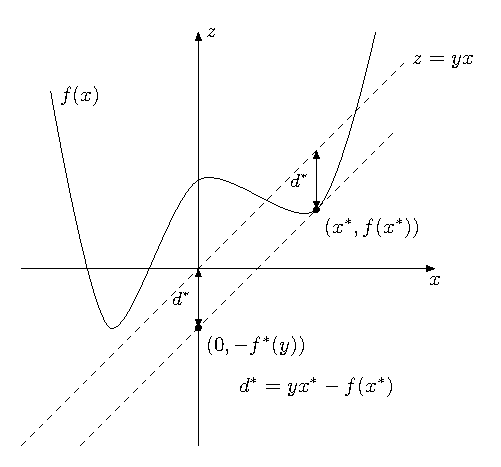
\includegraphics[scale=1]{geom.pdf}
\end{figure}
\end{frame}

\begin{frame}{Examples}
\begin{enumerate}
\item Linear function: $f(\bx) = \ba^{\T}\bx + b$
\item Negative entropy: $f(x) = x\log x$
\item Indicator function of the set $S$: $I_S(x) = 0$ iff $x \in S$
\item Norm: $f(\bx) = \|\bx\|$.
\item Squared norm: $f(\bx) = \frac{1}{2}\|\bx\|^2$
\end{enumerate}
\end{frame}

\begin{frame}{Calculus rules}

\begin{itemize}
\item Separable sum: $f(x_1, x_2) = g(x_1) + h(x_2)$ and $f^*(y_1, y_2) = g^*(y_1) + h^*(y_2)$
\item Translation of argument: $f(\bx) = g(\bx - \ba)$ and $f^*(\by) = \ba^{\T}\by + g^*(\by)$
\item Composition with linear invertible mapping: $f(\bx) = g(\bA\bx)$ and $f^*(\by) = g^*(\bA^{-\T}\by)$
\item Infimal convolution:  $f(x) = (h \square g)(x) = \inf\limits_{u + v = x} (h(u) + g(v))$ and $f^*(y) = h^*(y) + g^*(y)$
\end{itemize}

\end{frame}

\begin{frame}{Moreau-Yosida envelope}
\begin{itemize}
\item $f(\bx)$ is convex, but \emph{non-smooth}
\item Moreau-Yosida envelope ($\lambda > 0$)
\[
M_{\lambda f}(\bx) = \inf\limits_{\bu} (f(\bu) + \frac{1}{2\lambda}\|\bx - \bu\|^2_2) = \left(f \square \frac{1}{2\lambda} \|\cdot\|_2^2\right)(\bx)
\]
\item Huber function~-- $M_{\lambda f}$ for module
\begin{itemize}
\item $f(x) = |x|$
\item $M_{\lambda f}(x) = 
\begin{cases}
\frac{x^2}{2\lambda} & |x| \leq \lambda\\
|x| - \lambda / 2 & |x| \geq \lambda
\end{cases}$
\end{itemize}
\begin{block}{Exercise}
\begin{itemize}
\item Draw in the one figure $f(x)$ and $M_{\lambda f}(x)$
\item Derive expression of $M_{\lambda f}$ for $f(\bx) = \|\bx\|_1$ 
\end{itemize}
\end{block}
\end{itemize}

\end{frame}

\begin{frame}{Why do we get smooth function?}
\begin{itemize}
\item $M_{\lambda f}(\bx)$~-- convex
\item $M^*_{\lambda f}(\by) = f^*(\by) + \frac{\lambda}{2}\|\by\|_2^2$~-- strongly convex with parameter $\lambda$
\item $M_{\lambda f} = M^{**}_{\lambda f} = (f^* + \frac{\lambda}{2}\|\cdot \|_2^2)^*$
\item Conjugate function of the strongly convex function is smooth $\Rightarrow M_{\lambda f}$~-- smooth and 
\[
M'_{\lambda f}(\bx) = \frac{1}{\lambda} (\bx - \bu^*), \quad \bu^* = \argmin_{\bu} \left(f(\bu) + \frac{1}{2\lambda}\|\bx - \bu\|^2_2\right) 
\]
\end{itemize}

\begin{block}{Important property}
Sets of minimizers of $f$ and $M_{\lambda f}$ are the same.
\end{block}

\end{frame}

\begin{frame}{Recap}

\begin{itemize}
\item Conjugate functions
\item Young-Fenchel inequality and other properties
\item Smoothing of non-smooth functions
\item Examples
\end{itemize}

\end{frame}

\end{document}